\documentclass[12pt]{article}
\usepackage[margin=2.5cm]{geometry}
\usepackage{enumerate}
\usepackage{amsfonts}
\usepackage{amsmath}
\usepackage{fancyhdr}
\usepackage{amsmath}
\usepackage{amssymb}
\usepackage{amsthm}
\usepackage{mdframed}
\usepackage{graphicx}
\usepackage{subcaption}
\usepackage{adjustbox}
\usepackage{listings}
\usepackage{xcolor}
\usepackage{booktabs}
\usepackage[utf]{kotex}
\usepackage{hyperref}

\definecolor{codegreen}{rgb}{0,0.6,0}
\definecolor{codegray}{rgb}{0.5,0.5,0.5}
\definecolor{codepurple}{rgb}{0.58,0,0.82}
\definecolor{backcolour}{rgb}{0.95,0.95,0.92}

\lstdefinestyle{mystyle}{
    backgroundcolor=\color{backcolour},
    commentstyle=\color{codegreen},
    keywordstyle=\color{magenta},
    numberstyle=\tiny\color{codegray},
    stringstyle=\color{codepurple},
    basicstyle=\ttfamily\footnotesize,
    breakatwhitespace=false,
    breaklines=true,
    captionpos=b,
    keepspaces=true,
    numbers=left,
    numbersep=5pt,
    showspaces=false,
    showstringspaces=false,
    showtabs=false,
    tabsize=1
}

\lstset{style=mystyle}

\pagestyle{fancy}
\renewcommand{\headrulewidth}{0.4pt}
\lhead{CSC 343}
\rhead{Worksheet 1}

\begin{document}
\title{CSC343 Worksheet 1}
\maketitle

\noindent \textbf{Note:} This is student designed study guide to make learnings easier.
This does not reflect the course material. Please take it only as a reference.

\begin{enumerate}[1.]
    \item \textbf{Exercise 2.4.2:} Draw expression trees for each of your expressions
    of Exercise 2.4.1

    \item \textbf{Exercise 2.4.3:} This exercise builds upon Exercise 2.3.2 concerning
    World War II capital ships. Recall it involves the following relations:


    Figures 2.22 and 2.23 give some same data for these four relations. Note that unlike
    the data for Exercise 2.4.1, there are some ``dangling tuples'' in this data,
    e.g. ships mentioned in \textit{Outcomes} that are not mentioned in \textit{Ships}.

    \bigskip

    Write expressions of relational algebra to answer the following queries. You
    may use the linear notation of Section 2.4.13 if you wish. For the data of Figs.
    2.22 and 2.23, show the result of your query. However, your answer should work
    for arbitrary data, not just the data of these figures.

    \bigskip

    \begin{enumerate}[a)]
        \item Give the class names and countries of the classes that carried guns
        of at least 16-inch bore.
        \item Find the ships launched prior to 1921.
        \item Find the ships sunk in the battle of the Denmark Strait.
        \item The treaty of Washington in 1921 prohibited capital ships heavier than
        35,000 tons. List the ships that violated the treaty of Washington.
        \item List the name, displacement, and number of guns of the ships engaged
        in the battle of Guadalcanal.
        \item List all the capital ships mentioned in the database. (Remember that all
        these ships may not appear in the \textit{Ships} relation).
        \item Find the class that had only one ship as a member of that class
        \item Find those countries that had both battleships and battlecruisers.
        \item Find those ships that ``lived to fight another day''; they were damanged
        one battle, but later fought in another
    \end{enumerate}

    \begin{center}
    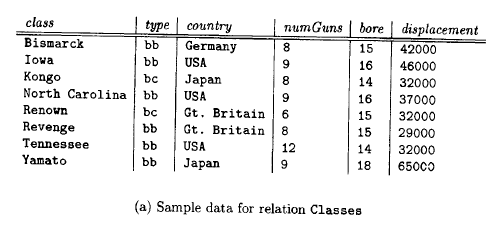
\includegraphics[width=0.75\linewidth]{images/worksheet_2_1.png}
    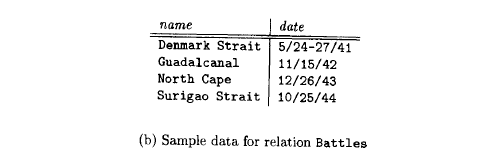
\includegraphics[width=0.75\linewidth]{images/worksheet_2_2.png}
    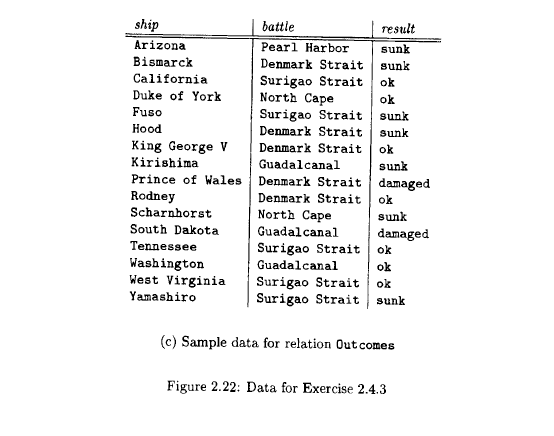
\includegraphics[width=0.75\linewidth]{images/worksheet_2_3.png}
    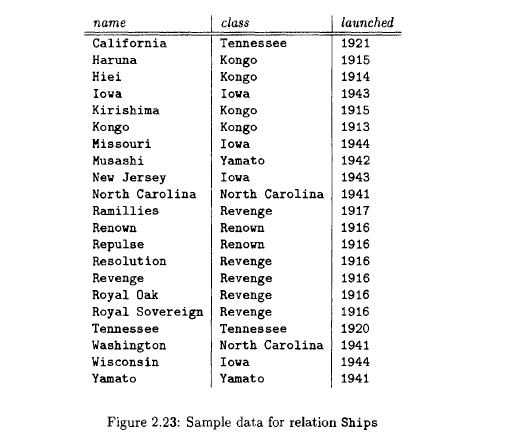
\includegraphics[width=0.75\linewidth]{images/worksheet_2_4.png}
    \end{center}

    \item \textbf{Exercise 2.4.4:} Draw expression trees for each of your expressions of
    Exercise 2.4.3

    \item \textbf{Exercise 2.4.5:} What is the difference between the natural join $R \bowtie S$ and the
    theta-join $R \bowtie_C S$ where the condition $C$ is that $R.A = S.A$ for
    each attribute $A$ appearing in the schemas of both $R$ and $S$
\end{enumerate}

\bigskip

\underline{\textbf{Reference}}

\bigskip

\begin{enumerate}[1)]
    \item Stanford: CS145 - Introduction to Databases, \href{http://infolab.stanford.edu/~ullman/fcdb/aut07/index.html}{link}
\end{enumerate}

\end{document}